% !TEX TS-program = pdflatex
% !TEX root = ../LightMicroRep.tex

%************************************************
\chapter{Deconvolution}
\label{chp:Deconvolution}
%************************************************
%\numberwithin{figure}{section}
%----------------------------------------------------------------------------------------
%	INTRODUCTION
%----------------------------------------------------------------------------------------

\section{Introduction}

\paragraph{Aim} To obtain/restore high resolution images using deconvolution methods. 
\\

High resolution microscopy is often plagued by blurriness due to diffractions (convolution). 
Inverse convolution (deconvolution) methods can be performed to obtain convolution-free images by describing a mathematical function called the Point Spread Function (PSF) to recalculate diffracted light, stray light, and out-of-focus light back to its origin~\cite{Lect10}.  

%----------------------------------------------------------------------------------------
%	METHODS
%----------------------------------------------------------------------------------------

\section{Methods}

Two samples, 200 nm Tetraspeck beads and \textit{Dictyostelium discoideum} cells (AX2 line) were used in this experiment. 
Deconvolution was performed using three methods; (constrained) iterative, fast iterative, and (regularized) inverse filter, each obtained by calculation of PSF from direct measurement in the experiment (measured/M) and through calculation from the parameters of the device (theoretical/T). 
To obtain the FWHM, a line profile measurement was done for each beads, for each channels. 
Afterwards procedures for gaussian fit and averaging were done in \faPython Python (script available publicly on \href{https://github.com/howset/LightMicro}{\faGithub~GitHub}, or by request).

%----------------------------------------------------------------------------------------
%	RESULTS AND DISCUSSION
%----------------------------------------------------------------------------------------
\section{Results and Discussion}

%--------------------------------------------
\subsection{Tetraspeck beads}

\begin{figure}
\centering
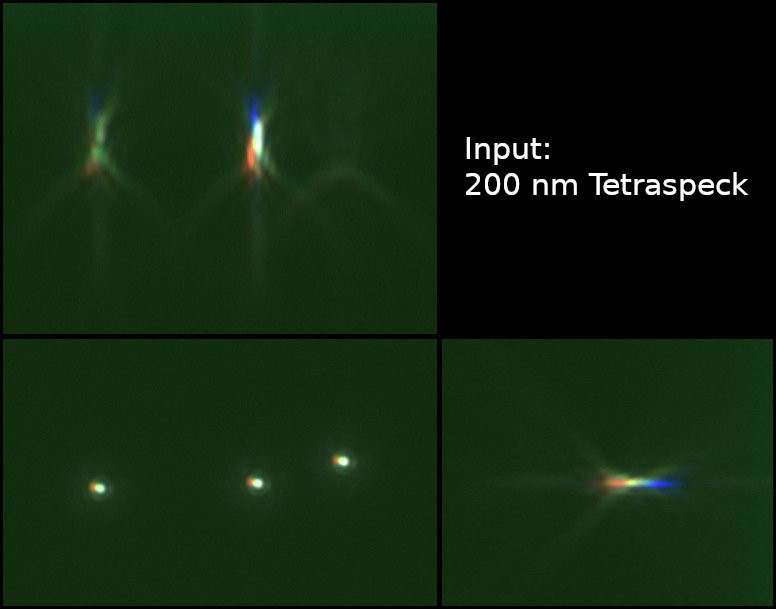
\includegraphics[width=.48\columnwidth]{Exp_7_Deconvolution/Figures/bcomposite/g_b_input}\\
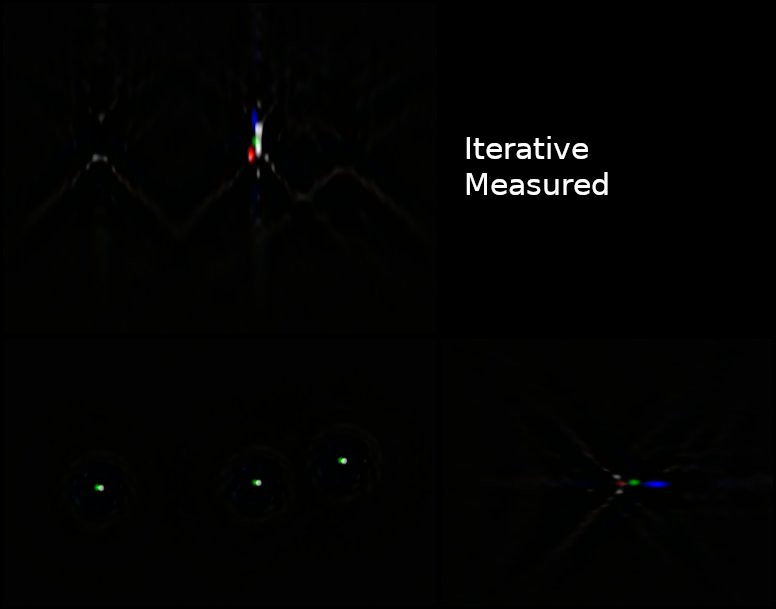
\includegraphics[width=.48\columnwidth]{Exp_7_Deconvolution/Figures/bcomposite/g_b_iterc}
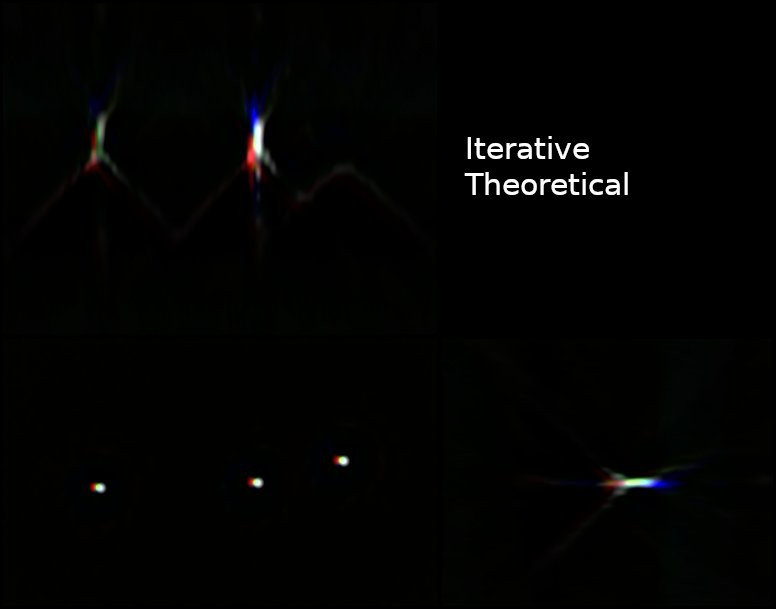
\includegraphics[width=.48\columnwidth]{Exp_7_Deconvolution/Figures/bcomposite/g_b_itert}\\
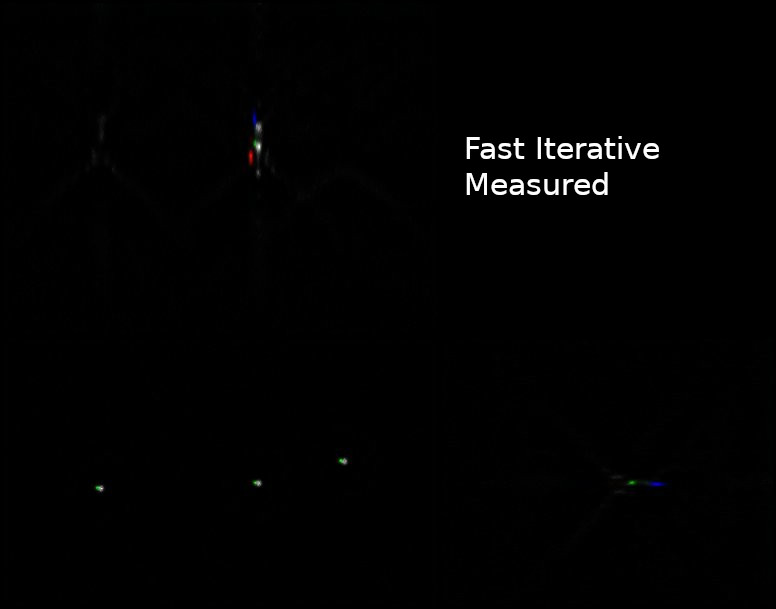
\includegraphics[width=.48\columnwidth]{Exp_7_Deconvolution/Figures/bcomposite/g_b_fastiterc}
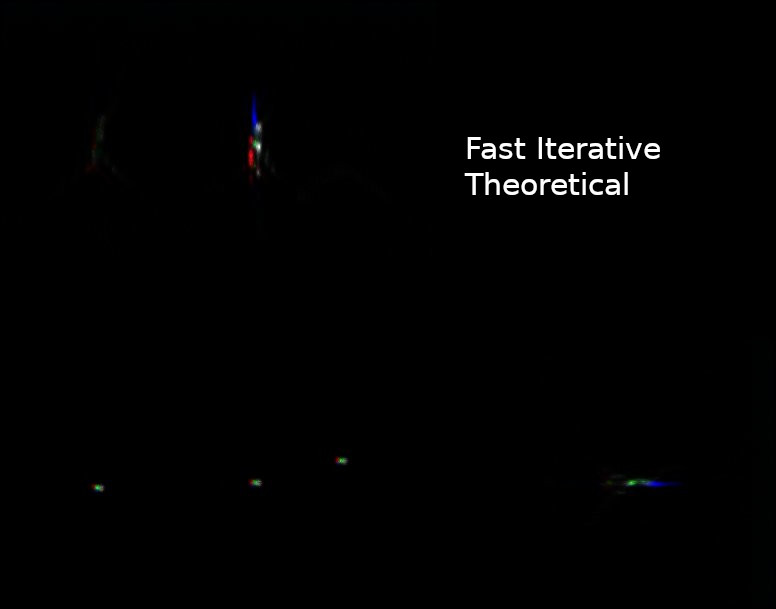
\includegraphics[width=.48\columnwidth]{Exp_7_Deconvolution/Figures/bcomposite/g_b_fastitert}\\
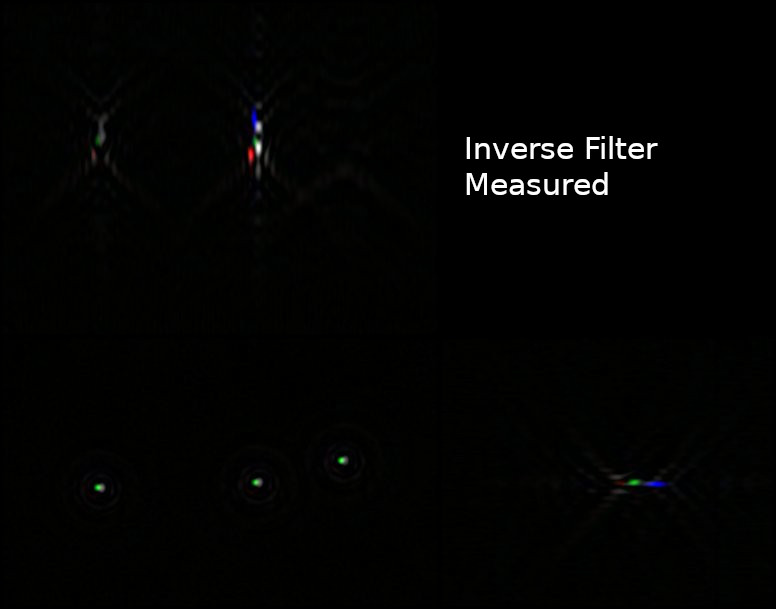
\includegraphics[width=.48\columnwidth]{Exp_7_Deconvolution/Figures/bcomposite/g_b_invfilc}
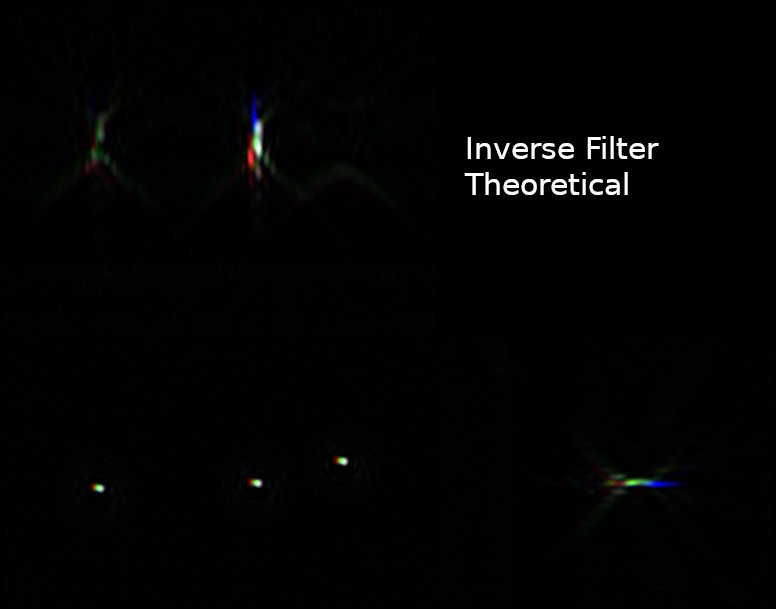
\includegraphics[width=.48\columnwidth]{Exp_7_Deconvolution/Figures/bcomposite/g_b_invfilt}\\
\caption{Orthoview of tetraspeck beads acquired raw (called input) and deconvoluted on 4 channels: red/orange, green, blue, and infrared/dark red. Objective lens: Plan Apochromat 100$\times$/1.4 Oil Ph3}
\label{fig:beads}
\end{figure}


The 200 nm Tetraspeck beads emit at four different wavelengths: 430 nm (blue), 515 nm (green), 580 nm (orange) and 680 nm (dark red)~\cite{Tetra}, these correspond to Ch3, Ch2, Ch1, and Ch4 in the case of this experiment. 
The beads were imaged as depicted in Fig.~\ref{fig:beads}. During the experiment, only three good beads that could be found. 
From the raw (input) image, a PSF was calculated (measured PSF). 
The PSF obtained in this way was then used for deconvolution purposes. Another PSF was calculated (theoretically) from various imaging parameters/device parameters and also used for deconvolution procedures (theoretical PSF) as a comparison. 

At first glance, it can be observed the various deconvolution methods (iterative, fast iterative, and inverse filter) performed differently, especially in the z-dimension. 
It can also be noticed that there is a different focus of the different channels, most prominently seen, again, in the z-dimension. 
The shift could be caused by chromatic abberations. 
This shift in focus that can be seen on all images could also be caused by movement of the filter carousel when changing measurement channel during imaging that does not retain the same original focus. 
Another immediate observation shows that the green channel exhibit a relatively rough background noise which is typical (not shown).

Comparing the measured deconvolutions and the theoretical ones, it is immediately obvious that the resolution in the z-dimension of the measured is better than the theoretical. 
Calculating the FWHM of each deconvolution methods would give a better overview of their performance in the xy-dimension. 
This is done by taking a line profile (intensity profile) of all acquired beads on all channels, then make a gaussian fit of the intensity profile and calculate the average FWHM.
In principal, the resolution in z-dimension can also be obtained in a similar way, however the difference would seem that in this dimension, the object would be in a different shape (more elongated), and also consequently the intensity profile should be taken along the z-axis.

The gaussian fits were first performed using an offset parameter due to the presence of measurements that seems to be off the baseline (channel 2 of the input image). 
However this seems to set the gaussian fit to fail on some other measurements. 
Adjusting the initial guess of this parameter (and also the others: A, $\mu$, and $\sigma$) seems to remedy the failure on these measurements, however it would then arbitrarily cause failure on completely different measurements. 
Since no pattern or explanation could be obtained, it was then decided to make a baseline correction to the initially problematic measurements, namely channel 2 of the input image by substracting the intensity values with the minimum value which provides the baseline of around 0, putting them on the same baseline level as the other measurements. 
This allows for the removal of the offset term of the fit and resulted in the successful application of the whole fitting procedure. 
It is probably also worth mentioning that no intensity normalization was conducted due to the fact that the fit at this point seems fine already.

The result of this is given in Tab.~\ref{tab:avfwhm} and visualized in a barplot in Fig.~\ref{fig:avfwhmbar}. 
It can be seen here, that the FWHM of the input image is naturally the largest, due to the fact that no deconvolution procedure was performed. 
The FWHM of the input image is around 30\% larger than the actual size of the beads (200 nm), and all attempts of the deconvolution procedures managed to bring the FWHM lower. 
It can be concluded that all methods using measured PSF consistently performs better on all channels than methods using theoretical PSF except in the case of measurement of fast iterative method on channel 4 where the values are really close. 
And among the three deconvolution methods, fast iterative constantly yields the smallest FWHM on all channels.

\begin{table}[h!]
\caption{FWHM\textsuperscript{+} for Tetraspeck beads}
\begin{center}
\begin{tabular}{cccccccc}
\toprule
 & \thead{\scriptsize{Input}} & \thead{\scriptsize{Inverse}\\\scriptsize{Filter (T)}} & \thead{\scriptsize{Inverse}\\\scriptsize{Filter (M)}} & \thead{\scriptsize{Iterative}\\ \scriptsize{(T)}} & \thead{\scriptsize{Iterative}\\ \scriptsize{(M)}} & \thead{\scriptsize{Fast}\\\scriptsize{Iterative (T)}} & \thead{\scriptsize{Fast}\\\scriptsize{Iterative (M)}}\\
\midrule
\scriptsize{Ch1}&\scriptsize{347.10(6.18)}& \scriptsize{231.22(1.81)}&\scriptsize{214.64(1.12)}&\scriptsize{290.29(0.15)}&\scriptsize{230.56(2.12)}&\scriptsize{188.48(9.44)}&\scriptsize{149.50(2.50)}\\
\scriptsize{Ch2}&\scriptsize{301.83(2.90)}& \scriptsize{226.78(1.65)}&\scriptsize{209.23(4.25)}&\scriptsize{246.10(2.32)}&\scriptsize{198.97(2.90)}&\scriptsize{182.06(19.87)}&\scriptsize{145.06(13.58)}\\
\scriptsize{Ch3}&\scriptsize{334.31(4.84)}& \scriptsize{206.58(1.67)}&\scriptsize{183.41(1.32)}&\scriptsize{282.08(2.94)}&\scriptsize{211.90(4.84)}&\scriptsize{171.34(3.06)}&\scriptsize{127.85(2.56)}\\
\scriptsize{Ch4}&\scriptsize{388.33(3.65)}& \scriptsize{245.41(0.87)}&\scriptsize{228.45(2.97)}&\scriptsize{300.79(0.95)}&\scriptsize{212.87(3.65)}&\scriptsize{184.99(4.76)}&\scriptsize{185.11(4.69)}\\
\bottomrule
\end{tabular}
\label{tab:avfwhm}
\end{center}
\scriptsize{\textsuperscript{+}Given in nm (average of the three present beads), standard deviation in parenthesis. (M) means the PSF is acquired by measurement, and (T) means the PSF is acquired by theoretical calculations of imaging parameters. Ch1 is red/orange (580 nm), Ch2 green (515 nm), Ch3 is blue (430 nm), and Ch4 is infrared/dark red (680 nm).}
\end{table}

\begin{figure}[h!]
\centering
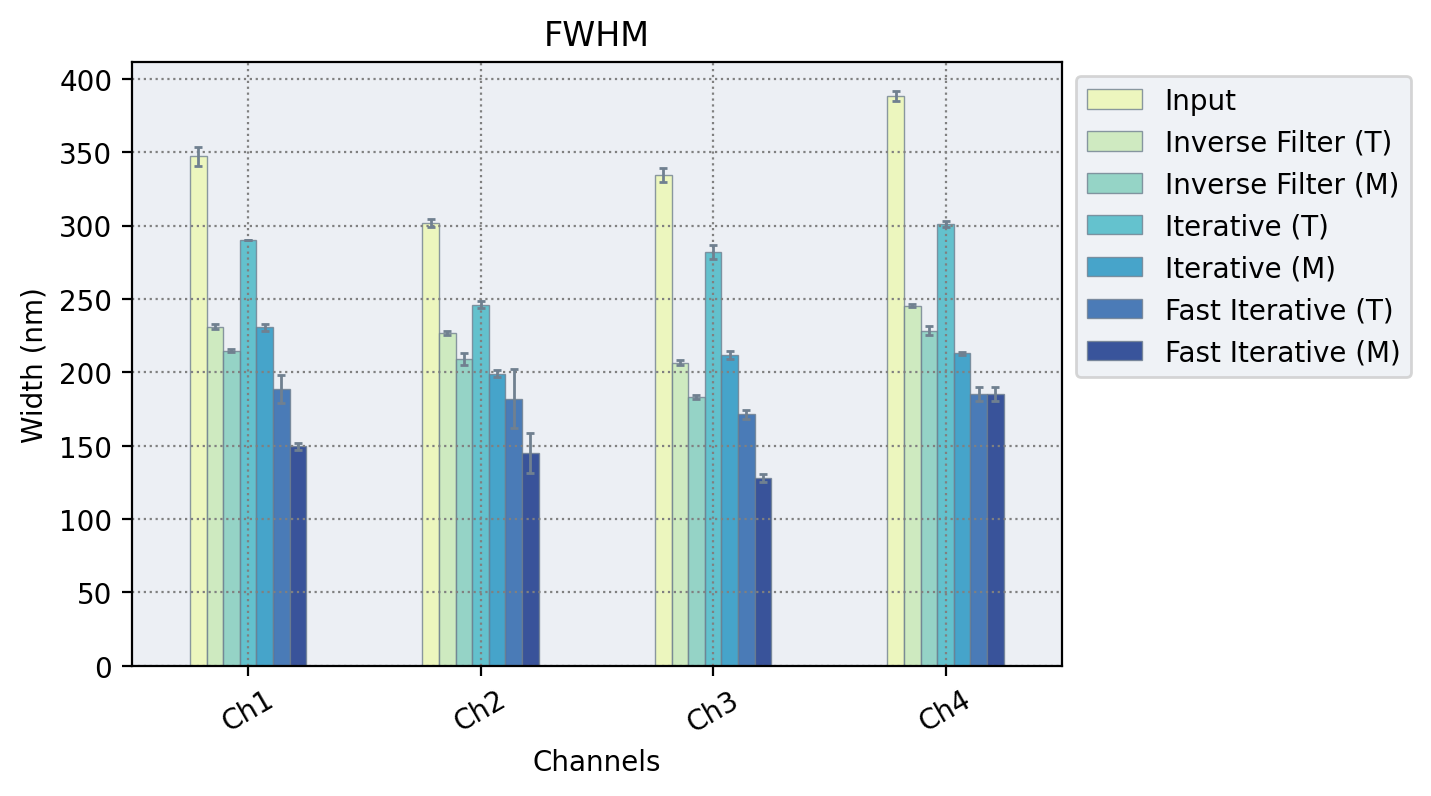
\includegraphics[width=.9\columnwidth]{Exp_7_Deconvolution/Figures/av_tabnmerr7}\\
\caption{FWHM of Tab.~\ref{tab:avfwhm} in barplot with the standard deviation given as error bars.}
\label{fig:avfwhmbar}
\end{figure}

The optical resolution following the Rayleigh criterion, given by $d=0.61\times(\lambda/NA)$, where $d$ is the minimum distance where two points are resolved, $\lambda$ is the wavelength of illumination, and $NA$ is the numerical aperture of the lense, yield for each channel 1-4 (i.e. red/orange, green, blue, and dark red/infrared): 252.71 nm, 224.39 nm, 187.35 nm, and 296.28 nm respectively. 
Given that the minimum distance for two points to be considered resolved is where the maximum of one point is directly on the first minimum of the other peak ($\approx$ FWHM), it seems that at least in the xy-dimension, the calculated FWHM of all deconvolution methods at all considered channels does not correspond all that well with the Rayleigh criterion.
 
Although in principal, it is known that the iterative method should give the best resulting image quality because of its ability to calculate light from various focal planes back to its place of origin, with the disadvantage being that it may take a long time for this deconvolution method to be performed due to the number of iterations in performing deconvolution algorithm (40 in this case). 
The fast iterative method is basically the same with the limitation on the number of iterations. 
The inverse filter is a method that involves a Fourier transformation and is the fastest method among these three.


%--------------------------------
\subsection{AX2 cells}

The PSF obtained from previous experiment on tetraspeck beads was then used for the deconvolution of AX2 cells images. Shown in Fig.~\ref{fig:ax2mon}~(Left). 
The following organelles are labelled: nucleus by DAPI, CP91 (core of centrosome) by anti-rabbit-AlexaFluor568, and CP224 (corona of centrosome) by anti-mouse-AlexaFluor488.

\begin{figure}
\centering
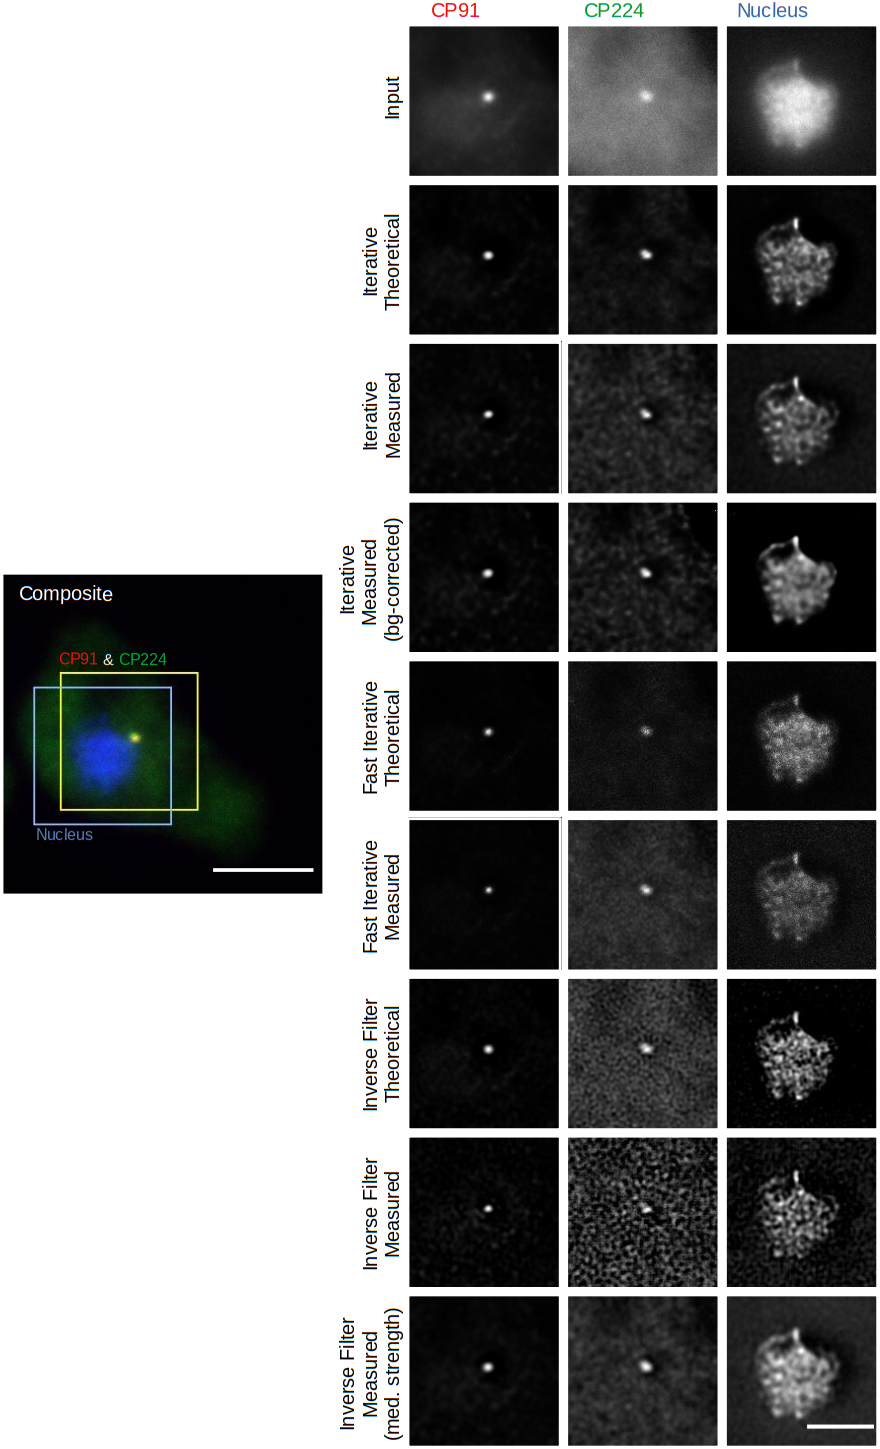
\includegraphics[height=0.85\textheight]{Exp_7_Deconvolution/Figures/montagemerged3t}\\
\caption{Objective lens: Plan Apochromat 100$\times$/1.4 Oil Ph3. \textbf{Left}: The composite of single representative optical sections of a z-stack of the raw input image of AX2 cells. CP91 is labelled by AlexaFluor-568 (red), CP224 by AlexaFluor-488 (green), and the nucleus by DAPI (blue). 
Gamma correction of 1.50 was applied on all channels of the composite for visualization purposes. 
Yellow square marks the cropped area on CP91 and CP224 channel on the right montage, blue square marks the cropped area on the nucleus channel. 
Scale bar is 5 $\mu$m. \textbf{Right}: A montage of the resulting deconvolution process. 
Each image shown here corresponds to the optical section shown on left image. 
No gamma correction. 
Scale bar is 3 $\mu$m.}
\label{fig:ax2mon}
\end{figure}

A montage image of each organelle according to the deconvolution methods is shown in Fig.~\ref{fig:ax2mon}~(Right). 
It can be seen that most deconvolution methods bring better image results in comparison to the raw/input image where contrasts are improved and structures are more readily recognizable. 
The size of CP91 is shown to be the smallest for the fast iterative method in comparison to other methods. 
This is consistent with the result from the discussion above where this deconvolution method yields the smallest FWHM. 

The iterative method with measured PSF produces a good CP224 images along with the vague fluorescence signals of AlexaFluor-488 bound to the $+$ ends of the microtubules. 
This feature can also be observed with the fast iterative method using measured PSF, though very vague, and seems absent in the method using theoretical PSF for both iterative and fast iterative. 
The inverse filter method seem to produce a mottling artifact in this channel. 
A mottling artifact is a phenomenon where signals, particularly noise in the background gets amplified by deconvolution algorithms. 
This phenomenon occurs usually with inversion algorithms, but iterative algorithms are also not free from this~\cite{DecArtif}. 

Inspecting the DAPI channel, it can be easily seen that the fast iterative method produces a much grainier image in comparison to the iterative method, both for the theoretical and measured PSF. 
This occurs on both previous channels of this method as well, just more prominently displayed here. 
This can be attributed to the limited number of iterations used in this method in comparison to the iterative method. 
The resulting images from the inverse filter method show, again, an artifact, which is arguably a ringing artifact. This artifact has an appearance of dark ripples around bright features of an image~\cite{DecArtif}.  

As a comparison, another set of images were also acquired for the iterative method using measured PSF, however this time using background correction. 
This acquisition shows a better form of the nucleus in the DAPI channel but does not seem to introduce major improvements for the other two channels in this observation. 
Another voluntary acquisition was also conducted for the inverse filter method using measured PSF. 
This time the artifacts appear less prominent and the images look more appropriate.

For the most part, the ability of the methods employed to restore images has a lot to do with the PSF itself and the raw image being restored, in regards that the PSF that is used should match the corresponding image. 
If there are aberrations in the image, then the PSF should also contain a corresponding aberrations as well. 
Otherwise, the deconvolved image may contain errors or be poorly restored~\cite{DecArtif}. 
Managing appropriate settings during image acquisitions also plays a major role.

%----------------------------------------------------------------------------------------
%	BIBLIOGRAPHY
%----------------------------------------------------------------------------------------

\renewcommand{\refname}{\spacedlowsmallcaps{References}} % For modifying the bibliography heading

%\bibliographystyle{unsrt}

%\bibliography{sample.bib} % The file containing the bibliography

